\documentclass[12pt]{article}

\usepackage{sbc-template}

\usepackage{graphicx,url}
\graphicspath{{img/}}

%\usepackage[brazil]{babel}   
\usepackage[utf8]{inputenc}  

\sloppy

\title{NoSQL - Armazenamento e Recuperação de Dados Não-Relacionais}

\author{Bruno Santos de Lima\inst{1}, Leandro Ungari Cayres\inst{1} }


\address{Faculdade de Ciências e Tecnologia\\
  Universidade Estadual Paulista \\
  "Júlio de Mesquita Filho" \\
  Caixa Postal 19060-900  -- Presidente Prudente -- SP -- Brasil
  \email{brunoslima4@gmail.com, leandroungari@gmail.com}
}

\begin{document} 

\maketitle

\begin{abstract}

Through growing technology of recent years, new concepts for data storage and manipulation have emerged, the traditional relational database model has dominated this area; but new applications require greater flexibility for data storage and retrieval, such features that are not fully provided by traditional database models, so this article is focused on describing non-relational databases, also known such as NoSQL, which are alternatives to relational databases and have been gaining more and more space in the technology environment in many types of applications.

\end{abstract}
     
\begin{resumo} 

Com a crescimento tecnológico dos últimos anos, novos conceitos para armazenamento e manipulação de dados surgiram, o tradicional modelo de banco de dados relacional tem dominado esta área; porém novas aplicações necessitam de uma maior flexibilidade para armazenamento e recuperação de dados, tais características que não são providas em sua totalidade por modelos de banco de dados tradicionais, assim este artigo está focado na descrição acerca de bancos de dados não-relacionais, também conhecidos como NoSQL, que são alternativas aos bancos de dados relacionais e vem ganhando cada vez mais espaço no meio tecnológico em diversos tipos de aplicações.

\end{resumo}

\section{Introdução}
\label{sec:intro}

Irrefutavelmente, é possível notar o avanço tecnológico e consequentemente, o crescimento do número de dispositivos eletrônicos, sejam supercomputadores, computadores pessoais ou dispositivos móveis, tornando-se cada vez mais presentes nas mais variadas situações do dia a dia, nos quais acelerômetros e giroscópios que antes inovações se tornaram sensores comuns, buscam obter e manipular diversos tipos de dados referentes a cada aplicação específica de um determinado contexto.

Em relação a manipulação de dados, com a presença diversas aplicações e dispositivos atuando a todo momento, torna-se necessário o armazenamento de forma a visar a integridade e consistência desse crescente volume de dados, que posteriormente possibilite abstrair informações relevantes sobre um determinado contexto, de forma a construir um montante de conhecimento e empregá-lo em prol de um propósito específico. O suporte automatizado para o armazenamento e manipulação de dados é provido por um Sistema de Banco Dados.

Quando o assunto Banco de dados é abordado logo é pensado como os dados não armazenados e manipulados? Para isso é seguido um modelo, de certa forma uma padronização, para responder esta pergunta, o modelo mais conhecido e utilizado em larga escala por Sistemas Gerenciadores de Banco de Dados (SGBD) é denominado modelo relacional \cite{codd:1970} criado por Edgar Frank Codd em 1970, o modelo relacional substituiu o modelo anterior chamado de modelo hierárquico tornando-se um padrão referência para este quesito, sendo utilizado pela grande maioria dos SGBD's, onde podemos citar por exemplo os mais conhecidos atualmente: MySQL, Oracle, SQL Server e PostgreSQL.\cite{brito2010bancos}

Contudo, atualmente o modelo relacional não provém a flexibilidade necessária que o cenário atual exige, principalmente em ambientes de \textit{Big Data}, e tem sido substituído em algumas áreas pelos chamados Bancos de Dados Não-Relacionais, ou NoSQL, este artigo tem como foco abordar o modelo não-relacional apresentando suas características, formas de armazenamento e recuperação dos dados, além de alguns contrastes ao modelo relacional.

Este artigo está organizado como segue: na Seção \ref{sec:nosql} é apresentado o conceito de banco de dados não relacional, a Seção \ref{sec:categorizacao} envatiza as categorias, ou seja, os tipos de NoSQL, os principais bancos de dados não-relacionais são descritos na seção \ref{sec:sistemas}, em seguida a Seção \ref{sec:vantagensedesvantagens} ressalta um comparativo entre banco de dados relacionais e NoSQL, por fim a Seção \ref{sec:estudoDeCaso} relata um estudo de caso desenvolvido na UFSCar que realiza uma análise de desempenho entre bancos de dados não relacionais e um banco de dado relacional.

\section{NoSQL} 
\label{sec:nosql}

%Com o decorrer do tempo foi pensado em modelagens alternativas ao tão utilizado modelo relacional, tais pensamentos justificam-se devido a algumas limitações presente no modelo relacional, limitações essas relacionadas a falta de flexibilidade fornecida pelo modelo relacional.
Desde a sua criação, na década de 1970, o modelo relacional tem imperado, sendo utilizado em larga escala pela maioria dos sistemas gerenciadores de banco de dados. Porém devido ao crescimento do número de aplicações e recursos que tem sido utilizados pelos atuais sistemas computacionais, a utilização de SGBDs tem se apresentado problemática e ineficiente, em decorrência de dificuldades com escalabilidade, particionamento de dados em um sistema distribuído; neste ponto se concentra uma solução alternativa.

O NoSQL foi idealizado em 1998, tem como significado de seu termo \textit{"Not Only SQL"}, ou seja, não apenas SQL, de forma a surgir como uma alternativa, possibilitando a coexistência de ambos, cada qual em seu espaço de atuação, priorizando a maior viabilidade. Por exemplo em aplicações distribuídas, como em redes sociais tais como Facebook e Twitter, as quais podem acumular \textit{terabits} de dados todos os dias, não existindo um esquema fixo, assim para este tipo de aplicação o NoSQL é mais vantajoso.\cite{gueidi:2016} 

Os banco de dados não-relacionais fornecem mecanismos de armazenamento e recuperação de dados que são modelados sob uma perspectiva não estruturada, diferentemente da forma disposta por tabelas e tuplas utilizada pelo modelo relacional \cite{zhaoSchema:2014}, sendo esta a sua principal característica do NoSQL, a ausência de um esquema pré-definido, porém seu conceito é muito mais amplo, possibilitando a existência características peculiares a cada banco de dados NoSQL.

Abaixo estão descritas algumas características presentes em banco de dados não-relacionais:

%corrigir
\begin{itemize}
	\item Distribuído: os banco de dados não-relacionais são em geral distribuídos, assim várias máquinas são responsáveis por armazenar e prover esses dados quando os mesmos forem requisitados.\\
	\item Escalabilidade horizontal: está relacionado a distribuição do banco de dados em várias máquinas paralelamente, realizando um conjunto de atividades, este conceito está fortemente ligado o aplicações distribuídas. \\
	\item Grande volume de dados: Um dos propósitos do NoSQL é ter a capacidade de armazenamento de grandes volumes de dados sem grandes perdas de desempenho.\\
	\item SQL não é suportado: De uma modo geral nos banco de dados NoSQL não é utilizado a linguagem SQL, assim cada sistema tem seu próprio modo de realizar consultas, através de uma sintaxe própria ou utilização de \textit{drivers} para linguagens de programação.\\
	\item BASE: Conceito oposto ao ACID, o BASE é um conceito presente em todos os sistemas de banco de dados não-relacionais, associando características de disponibilidade, estado leve e eventual consistência. A abordagem ACID e BASE serão confrontadas com maiores detalhes na seção \ref{sect:acid}.
\end{itemize}

\section{Categorização dos Banco de dados NOSQL}
\label{sec:categorizacao}


O NoSQL pode ser classificado em cinco categorias \cite{typeNOSQL:2013} sendo estas: 

\begin{itemize}
\item Armazenamento chave-valor: esta abordagem trabalha com duas informações associadas a um registro, a primeira consiste na chave e a outra o valor, este segundo consiste literalmente no dado armazenado, como isso seu mecanismo de funcionamento atua de forma similar a um \textit{Hash Table}, permitindo acesso rápido, alta concorrência e armazenamento em massa, porém o grande ponto negativo deve-se a falta de uma esquematização o que deixa a visualização da organização desses dados dificultada.\cite{typeNOSQL:2013}\\

\item Orientação a colunas: esta técnica visa organizar os dados em colunas, ou seja, ocorre uma mudança de orientação agora por atributos, colunas, e não mais por registros, tuplas. Dois exemplos dessa categoria de banco de dados orientado por colunas é o Cassandra e o BigTable.\cite{brito2010bancos}\cite{surveyNosql:2012}\\

\item Orientação a documentos: nesta abordagem os dados são armazenados na forma de documentos textuais associados a uma chave única, a qual representa a localização de armazenamento, que em geral é fornecida por uma API ou uma linguagem de consulta para que esses documentos possam ser recuperados rapidamente. \cite{surveyNosql:2012} Uma vantagem relacionado a essa categoria está no aproveitamento de espaço de armazenamento, visto que um documento tem um tamanho necessário para armazenar os dados em que nele estão sem que ocorra desperdício de espaço, sem atributos vazios ou nulos, um dos principais representantes deste modelo é o MongoDB. Esse modelo deve ser evitado em aplicações que envolvem muitos relacionamentos.\cite{typeNOSQL:2013}\\

\item Orientação a grafos: nesta técnica o armazenamento é baseado em grafo, em que cada nó é um objeto e o relacionamento entre esses objetos é expresso pelas arestas que ligam dois nós. Esse tipo de modelo é indicado para redes sociais, sistemas bioinformática entre outros, pois os nós podem representar por exemplo pessoas, entretanto é importante ressaltar que o aumento na complexidade do agrupamento de dados é diretamente proporcional ao número de registros.\cite{typeNOSQL:2013}\cite{surveyNosql:2012} \\

\item Orientação a objetos: nesta abordagem os dados são armazenados na forma de objetos, objetos análogos aos do paradigma de programação orientado a objetos oferecendo recursos como encapsulamento, polimorfismo e herança, cada objeto tem um identificador único que representa o objeto unicamente.\cite{typeNOSQL:2013}\\

\end{itemize}

Adicionalmente, têm sido elaborados banco de dados não-relacionais híbridos, de forma a serem compostos por mais de uma destas abordagens, buscando usufruir das vantagens de cada categoria e amenizar o ônus de utilização. 

\section{Principais sistemas de banco de dados não-relacionais}
\label{sec:sistemas}

Através de pesquisas desenvolvidas na área de banco de dados relacionais, principalmente pelas grandes empresas de tecnologia, diversos sistemas de banco de dados adquiriram destaque, a seguir serão apresentados os principais em breve histórico.

Em 2004, a partir da idealização e desenvolvimento da Google surge um banco de dados proprietário de alta performance chamado \textit{BigTable} que tinha como objetivo prover maior escalabilidade e disponibilidade não fornecida pelos banco de dados não relacionais.\cite{brito2010bancos}

Posteriormente, um sistema de destaque desenvolvido pela Amazon em 2007 foi chamado de \textit{Dynamo}, com características não-relacionais básicas provia alta disponibilidade sendo destinado para os \textit{web services} da própria Amazon.\cite{brito2010bancos}

Imediatamente a seguir, em 2008, a empresa Facebook apresentou um dos principais sistemas de banco de dados da atualidade, chamado Cassandra, como um banco de dados não-relacional com fortes características de dados distribuídos e alta disponibilidade, sendo capaz lidar com grandes volumes de dados ideal para ambientes de Big Data, como sua rede social. O projeto foi tão bem sucedido que foi adotado pela rede social Twitter, em substituição ao MySQL.\cite{brito2010bancos}

Neste mesmo período, uma iniciativa da empresa Apache viabilizou o desenvolvimento do sistema denominado Apache CouchDB que é orientado a documentos, utilizando o mesmo princípio  de orientação a documentos. Em 2009, o sistema de banco de dados MongoDB foi apresentado sendo altamente escalável e possuindo características semelhantes ao CouchDB.\cite{brito2010bancos}

\section{Propriedades ACID e BASE}
\label{sect:acid}
Dentre os principais fatores que impactam negativamente sob o desempenho de banco de dados relacionais, estão todas as operações necessárias para garantir as características da propriedade ACID (Atomicidade, Consistência, Isolamento e Durabilidade), tais atributos garantem a independência e completa execução de transações, garantindo a integridade dos dados após sucessivas manipulações.\cite{brito2010bancos}

Perante este arcabouço de funcionalidades, que por um lado fornece consistência, por outro há grandes perdas de desempenho, os banco de dados não-relacionais baseiam-se em outro conjunto de propriedades chamado BASE (Disponibilidade básica, estado leve e consistência eventual). Devido estas propriedades, o banco de dados não necessita estar a todo momento consistência, mas somente nos devidos momentos, pode ter uma máquina inoperante que mesmo assim estará em funcionamento devido ao fácil escalonamento, desta forma, obtem-se ganhos de desempenho ao eliminar diversos funcionalidades que pesariam em comparação ao modelo relacional.\cite{brito2010bancos}


\section{Comparativo: Modelo Relacional x NoSQL}
\label{sec:vantagensedesvantagens}

Quando a viabilidade de migração de um banco de dados relacional em detrimento de uma abordagem não-relacional é avaliada, deve-se estabelecer de todas as vantagens e desvantagens de cada modelo, em relação aos principais aspectos de escalonamento, consistência e disponibilidade. A tabela abaixo estabelece esse comparativo:

\begin{table}[h]
\caption{Comparativo entre bases de dados relacionais e não-relacionais. \cite{brito2010bancos}}
\begin{center}
\begin{tabular}{p{2.7cm} | p{5cm} | p{5cm}}
\hline
Escalonamento & Possível, porém complexo devido o modelo estruturado, a adição de forma dinâmica de novas máquinas não é incorporada naturalmente. & Uma das principais vantagens desse modelo, pois não possui nenhum esquema pré-definido, possui maior flexibilidade o que favorece a inclusão transparente de outros elementos. \\
\hline
Consistência & O conjunto de regras de consistência presentes propiciam uma maior grau de rigor quanto à consistência das informações. & Realizada de modo eventual no modelo, se nenhuma atualização for realizada sobre o item de dados, todos os acessos a esse item devolvem o último valor atualizado.\\
\hline
Disponibilidade & Dada a dificuldade de se conseguir trabalhar de forma eficiente com a distribuição dos dados, esse modelo pode não suportar a demanda muito grande de informações do banco. & Outro fator fundamental do sucesso desse modelo, capacidade de distribuição dos dados propicia que um maior número de solicitações aos dados seja atendida por parte do sistema e que o sistema fique menos tempo indisponível.\\
\hline
\end{tabular}
\end{center}
\end{table}

%Como toda tecnologia, o NoSQL também apresenta um conjunto vantagens e desvantagens em sua utilização, é importante acrescentar que essas vantagens e desvantagens podem variar de acordo com a necessidade de uma aplicação ou organização, ou seja, dependendo do propósito da aplicação as desvantagens são minimizadas devido à grande parcela de benefícios, deve-se avaliar o custo/benefício. A seguir, são discutido algumas vantagens e desvantagens em sua utilização.

%\subsection{Vantagens}
%\label{subsec:vantagens}

%Os Bancos de dados NoSQL tem como sua grande vantagem o processamento mais rápidos dos dados que estão armazenados se comparado com os Bancos de dados Relacionais. O fator que torna o Banco de dados relacional mais lento em processamento é caracterizado pelas chamadas restrições ACID, cujo a sigla representa Atomicidade, consistência, isolamento e durabilidade. 

%Atomicidade significa que toda atualização é executada por completa ou não, já a consistência é o fato de toda transação estar proibida de quebrar as regras do banco de dados, isolamento deve-se ao fato de que cada aplicação faça transações de modo independente a outras aplicações que estão atuando em paralelo. Essas restrições são importantes no quesito precisão, porem se utilizadas causam uma perda de desempenho no processamento, o NoSQL não utiliza o suporte para as restrições ACID aumentando o seu desempenho de processamento.\cite{leavitt:2010}

%A não utilização das restrições ACID não torna o NoSQL um Banco de dados inconsistente ou inseguro, apenas diminui essas capacidades, porém não as elimina por completo devido a utilização da BASE como uma alternativa ao conjunto ACID.\cite{pritchett:2008}

%Um outro aspecto para o processamento mais rapído de dados nos Bancos de Dados NoSQL é a simplificação do modelo, ou seja, de um modo geral seus modelos são mais simples facilitando seu processamento. Outra vantagem interessante do NoSQL está na flexibilidade que o modelo prove, essa flexibilidade permite que as organizações e desenvolvedores utilizem seus aplicativos da forma que melhor atenda suas necessidades.\cite{leavitt:2010}

%\subsection{desvantagens}
%\label{subsec:desvantagens}

%O NoSQL apresenta ainda alguns desafios, sendo um deles a maior complexidade devido a não utilização de SQL, todos as consultas devem ser realizadas manualmente através da programação, esse fator pode não ser um problema em consultas simples, porém podem potencializar um problema para as tarefas mais difíceis. A falta de ferramentas para gerenciamento ou mesmo para utilização como suporte parte do cliente ainda é um problema, onde essa falta de ferramentas pode estar relacionado ainda ao desconhecimento da tecnologia que pode ser um outro problema.\cite{leavitt:2010}

%Devido a não utilização de restrições ACID quesitos como confiabilidade e a consitência tornam-se um problema em Banco de dados NoSQL sendo uma desvantagem, principalmente para certos tipos de aplicações como bancarias este modelo não é recomendado.\cite{leavitt:2010}

\section{Um estudo de caso: Avaliação de Desempenho}
\label{sec:estudoDeCaso}

Poucas análises e avaliações de desempenho foram aplicadas a bancos de dados não-relacionais, Renato Molina Toth da Universidade Federal de São Carlos, descreve, em seu artigo intitulado "Abordagem NoSQL - uma real alternativa" \cite{toth2011abordagem}, um estudo de caso de avaliação de desempenho realizado com base no serviço Yahoo! Cloud Serving, no qual visa utilizar este serviço aplicando distintos tipos de bancos de dados não-relacionais, de forma a elaborar um estudo comparativo entre estes.

Para o estudo de caso, foi elaborado um modelo de benchmark para a avaliação da latência através da carga de trabalho de requisições, em que uma aplicação Java foi desenvolvida para esta finalidade, ou seja, realizar um grande número de transações. O experimento é descrito em três parte sendo elas: a carga de trabalho, o experimento em si e por fim os resultados coletados.

A carga de trabalho consiste em escolher quais transações serão empregadas, ou seja, deve-se visar diferentes tipos de consultas na base de dados de forma a exigir o máximo dos bancos de dados sob análise. O experimento trás dois tipos de carga de trabalho, possuindo tanto consultas de armazenamento, ou seja escrita, quanto de recuperação, o qual refere-se a operação de leitura, além de considerar diferentes tamanhos de registros armazenados.

Os bancos de dados não-relacionais utilizados no estudo foram o \textit{Cassandra}, \textit{Hbase} e \textit{Sherpa}, as figuras a seguir mostram o desempenho desses bancos de dados, através da utilização de duas cargas de trabalhos pré-definidas. De forma complementar a análise, foi adicionado um banco de dados relacional, no caso \textit{MySQL}, de forma a viabilizar um comparativo adicional.

\begin{figure}[ht]
	\centering
	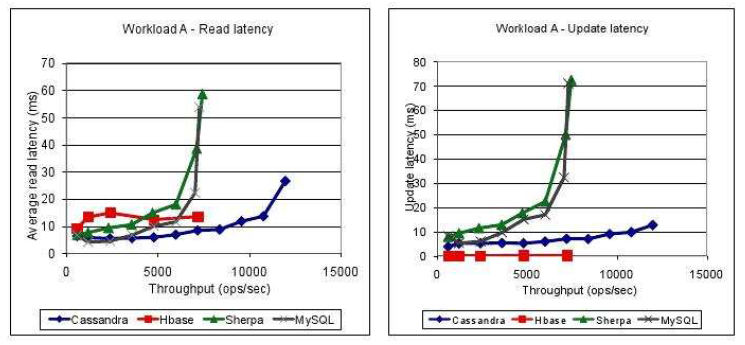
\includegraphics[width=.9\textwidth]{img/cargaA.png}
	\caption{Análise - Carga de trabalho A}
	\label{img:cargaA}
\end{figure}

\begin{figure}[ht]
	\centering
	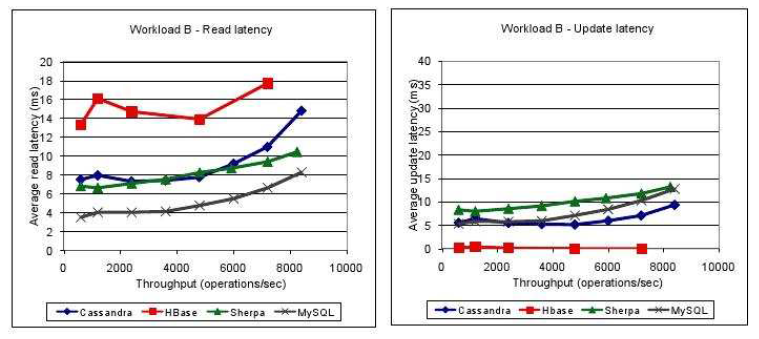
\includegraphics[width=.9\textwidth]{img/cargaB.png}
	\caption{Análise - Carga de trabalho B}
	\label{img:cargaB}
\end{figure}

Como resultados da análise, na carga de trabalho A podemos observar que o bancos de dados \textit{Cassandra} e \textit{HBase} demonstraram-se mais vantajosos para escrita tendo um maior desempenho e menor latência, porém o \textit{HBase} apresentou resultados inferiores no quesito leitura. Em relação a carga de trabalho B, os resultados apresentaram-se de forma similar, cujo destaque se refere ao banco de dados \textit{Sherpa}, o qual apresentou um ótimo desempenho em média para cargas de trabalho menores.

Como resultado, ainda foi possível constatar que que o banco de dados relacional teve uma performance constante, porém apresentando maior latência se comparado aos bancos de dados não-relacionais estudados principalmente após atividades de leitura. Como conclusão do estudo de caso, foi considerado que os bancos de dados NoSQL tiveram maior performance que o relacional na maioria dos casos.

\section{Conclusão}
\label{sec:conclusao}

Em suma, os banco de dados não-relacionais são atuais alternativas ao tradicional modelo relacional, acrescentando novos conceitos principalmente flexibilidade e escalabilidade, não presentes no modelo relacional e tão requeridas nas aplicações mais recentes tanto pela simplicidade quanto desempenho, cuja finalidade está em otimizar mesmo em detrimento de alguns aspectos que possam reduzir a consistência, pois nem todas as aplicações precisam de consitência elevada em todo momento, algumas aplicações precisam de maior liberdade para trabalhar com seus dados, pois tem propósitos diferentes para utilizá-los.

Outro aspecto relevante, embora existam poucos estudos comparativos entres os modelos de banco de dados relacional e não-relacional, o NoSQL consiste em uma tecnologia em ascensão que está invadindo o mercado, sendo apoiada pelas principais empresas de tecnologia no mundo, tais como Facebook, Twitter e Amazon, as quais tem aplicado cada vez mais recursos em pesquisas para o desenvolvimento de novas tecnologias em um mundo em que o fluxo de dados cresce a cada instante, no chamado \textit{BigData}, no qual cada dado pode fazer a diferença na criação de novos conhecimentos.

\bibliographystyle{sbc}
\bibliography{sbc-template}

\end{document}
